\documentclass{article}

\usepackage[utf8]{inputenc}
\usepackage[T1]{fontenc}
\usepackage[francais]{babel}
\usepackage{setspace}
\usepackage{hyperref}
\usepackage{graphicx}
\usepackage{minted}
\usepackage[center]{qtree}

\title{Réalisation d'un interprète Lisp en Python}
\author{}
\date{}


\begin{document}

\maketitle
% \onehalfspacing

\section{Avant-propos}
% raison d'être personnelle du projet et guide de lecture du rapport (1/2 page)

Dans le cadre de la session du cours d'algorithmique 2 (EDF3SA2A), j'ai développé un interprète pour le langage Lisp en Python. 
L'objectif visé étant d'en apprendre plus sur les processus de traitements informatiques en œuvre dans ce type de réalisation,
mais aussi sur le fonctionnement interne du langage Lisp, premier langage fonctionnel.
\paragraph{}
Le choix du langage Lisp a été dicté pour plusieurs raisons. 
Tout d'abord, Lisp est un langage réputé facile à interpréter, de par sa (relative) simplicité syntaxique.
Ensuite, Lisp est un langage que nous avons étudié en cours d'introduction aux langages fonctionnels, 
et s'avère être un outil de choix dans l'enseignement de la programmation et de l'algorithmique en général.
Et enfin, cet interpréteur a été conçu également afin de servir de base à un autre projet à vocation pédagogique (\emph{ConsMaster}).


\section{Introduction}
% résumé du rapport mettant en valeur les points les plus intéressants (1 à 2 pages)

Nous présentons dans ce document la réalisation d'un interprète Lisp minimaliste en Python 3, à l'aide de \emph{(Python Lex Yacc)}.
\\ 
L'interprète dont il est question dans ce document peut être récupéré en ligne à l'adresse \url{https://gitorious.org/pyLisp}.
\paragraph{}
Seront expliqué dans un premier temps les aspects généraux relatifs à la programmation d'un langage interprèté,
avec un focus sur un outil d'analyse lexicale et syntaxique disponible pour Python \emph{(Python Lex Yacc)}.
Ainsi, nous verrons quelles notions apprises en cours ont été utilisées, 
et nous discuterons de la pertinence d'une telle approche dans le cadre du langage Lisp.
\paragraph{}
Ensuite, nous discuterons des aspects techniques de l'interprétation dans un langage haut niveau comme Python,
en analysant les points forts et les points faibles de cette approche.
Je pense que l'approche orientée-objet s'est révélée être un outil précieux pour ce travail, ce point aussi sera donc élargi.
\paragraph{}
Nous aborderons également certaines problématiques spécifiques au langage Lisp, et leur solution dans notre travail.
Citons tout particulièrement les questions d'environnement, des modes de liaison, des appels de fonction 
(et tout particulièrement des formes spéciales), de la récursivité, du traitement des erreurs,
et du \emph{ramasse-miettes}.
La question des macros du langage Lisp sera aussi brièvement évoquée.
\paragraph{}
Chacune de ces parties sera illustrée dans la section implémentation par notre code source, 
éventuellement simplifié et enrichi d'explications, afin de donner un aperçu du travail concret qui a été effectué.
Toutefois, notre but n'est pas de présenter l'intégralité du code ici.


\section{Problématique}
% énoncer le problème à traiter, y compris ce qui n'a pas pu être fait. (idem) 
% expliquer les choix de ne pas faire telle ou telle partie

\subsection{objectifs}
Notre objectif étant d'avoir au final un interprète Lisp fonctionnel quoique minimaliste, tout en abordant les domaines 
essentiels de l’interprétation des langages, voici les objectifs que je me suis fixé :
\begin{enumerate}
  \item Disposer d'un interprète ayant la capacité de lire une expression Lisp correctement formée, 
  et la représenter en interne dans un format permettant son interprétation ;
  \item Permettre à l'interprète d'évaluer les expressions lues, et de retourner un résultat ;
  \item Permettre à l'interprète d'afficher le résultat de l'évaluation, et partant de pouvoir 
  afficher tout objet Lisp (y compris les objets circulaires) ;
  \item Pourvoir cet interprète des fonctions \emph{builtins} de base ;
  \item Permettre à l'utilisateur de définir de nouvelles fonctions et macros pour étendre le langage ;
  \item Que l'interprète ait les capacités de remonter les erreurs d’exécution dues au programmeur, 
  dans un format intelligible afin de faciliter la correction.
\end{enumerate}
\subsection{réserves}
Ces objectifs ont tous été atteints, avec toutefois quelques réserves :
\begin{itemize}
  \item Les fonctions builtins ont été uniquement mises en œuvre sur une petite vingtaine de fonctions comme \emph{Proof of Concept}.
  Par ailleurs, les fonctions d'\emph{entrée-sorties} principales (\emph{read} et \emph{print}) n'ont pas été réalisées 
  selon le modèle propre à Lisp 
	\footnote{La raison est que le modèle \{ lexer $\rightarrow$ parser $\rightarrow$ interprète \} que j'ai utilisé 
	ne s'y prête pas bien.}
  , et notre interprète est privé de capacités d'IO pour le moment.
  \item L'interprète ne dispose pas à ce jour de capacités de lire correctement les macro-caractères associés aux macros de Lisp, 
  faute de temps pour effectuer une gestion fine des macros Lisp. Néanmoins, un usage basique des macros reste possible.
  \item L'interprète n'a pas la capacité de lire une expression multiligne directement au \emph{toplevel}, 
  car il est difficile de déterminer quand lancer le parser.
  En revanche, le système de parsing est tout à fait capable d'évaluer un fichier source Lisp en entier.
\end{itemize}
\paragraph{}
Les deux faiblesses les plus handicapantes ont pour origine commune le fait d'avoir utilisé un système à base de 
\emph{lexer} et \emph{parser} pour le langage Lisp. 
Cette séparation du prétraitement de l'étape d'interprétation proprement dite rend l'ensemble beaucoup 
mois souple à gérer, et l'on m'a fait avec raison la remarque qu'il est inutile d'utiliser ce genre d'outils pour 
interpréter du Lisp, langage réputé simple à parser. 
Toutefois, cette approche ayant largement fait ses preuves pour la plupart des langages, il m'a paru dommage de ne pas explorer 
cette voie, ne serait-ce que pour son intérêt pédagogique.
\subsection{langage d'implémentation}
Pour ce qui est du choix du langage d'implémentation, je sais qu'il n'est pas courant d'écrire un interpréteur dans un langage
qui est lui même interprété, pour plusieurs bonnes raisons, essentiellement des questions de performances. 
Cependant, Python étant un langage très apprécié pour le prototypage, il m'a semblé raisonnable de l'utiliser pour ce projet.
\\
Une autre bonne raison étant que l'un des objectifs du projet était de pouvoir interfacer l'interprète 
avec le logiciel \emph{ConsMaster}, lui même écrit en Python.
\\
Disposer d'un langage de programmation orientée objet comme Python m'a également permis de structurer les objets Lisp 
comme une hiérarchie de classes, comme je détaillerais plus loin. Par ailleurs, le ramasse-miettes intégré à Python m'a permis
de ne pas me soucier de cet aspect, ce qui constitue un plus appréciable.

\section{Stratégies adoptées}
% comparaison aux traitements existants du même problème 
% (ici, les différentes stratégies d'implémentation et le choix fait, en l'expliquant) 3 à 4 pages

% Ici insérer partie sur algo 2

Lisp étant un langage relativement ancien, il en existe de multiples implémentations et même de multiples dialectes,
certaines implémentations étant même écrites en Lisp !
Notre implémentation n'a donc absolument pas la prétention d'apporter quelque chose de nouveau sur ce plan.
\\
Je n'ai malheureusement pas eu accès aux ouvrages de référence (j'ai entendu parler des livres de
\cite{allen_anatomy_1978} et \cite{queinnec_principes_2007} 
      \footnote{Le premier chapitre du livre de Christian Queinnec est disponible en ligne à l'adresse 
	  \url{http://paracamplus.com/Books/Cours/LiSP/4/extrait.pdf}.}
sur la question), 
donc je ne m'étendrai pas trop sur l'état de l'art dans le domaine, mais discuterai surtout ici 
des stratégies d'implémentation principales adoptées.
\paragraph{}
Il existe aujourd'hui un certain nombre de dialectes Lisp incompatibles entre eux.
Mon implémentation est fondée sur les connaissances acquises avec la manipulation de CLisp,
et mon choix s'est donc naturellement porté vers le dialecte Common-Lisp, simplifié à outrance.
\\
Parmi les parties que je n'ai pas effectué, citons notamment les objets d'IO, les paramètres
spéciaux pour les fonctions (\texttt{\&aux}, \texttt{\&optional}, \texttt{\&key}, \texttt{\&rest}...), 
la possibilité de créer des modules, etc.
En ce sens, mon Lisp s'apparente un peu à du Scheme pour l'aspect minimaliste.
\paragraph{}
On peut diviser les traitements effectués par un interprète Lisp standard en trois parties fondamentales :
\begin{enumerate}
  \item La fonction \emph{read}, qui permet de lire un objet Lisp sur un flux d'entrée, et de le représenter 
  en interne en vue de son traitement ;
  \item La fonction \emph{print}, qui permet d'afficher, et plus généralement d'envoyer sur un flux de sortie
  une représentation \emph{human-readable} de cet objet interne ;
  \item La fonction \emph{eval}, qui permet d'évaluer une expression Lisp comme une fonction, et de retourner
  un résultat.
\end{enumerate}
Le tout résumant fort bien le fonctionnement d'un interprète, avec la boucle
\texttt{(loop (print (eval (read))))}. Analysons étape par étape :

\subsection{read}
La plus simple (et probablement la meilleure) façon de réaliser la première partie est d'écrire une fonction
\emph{ad-hoc}, tant le langage Lisp est simple syntaxiquement. Néanmoins, j'ai favorisé une méthode plus compliquée,
mais aussi plus généraliste, celle d'utiliser un analyseur lexical et syntaxique.
\subsubsection{lexing}
Un lexer se contente d'analyser un code source, et de le ``découper'' en éléments lexicaux
correspondants à un langage donné. Cette étape, pour être menée à bien, doit être débarrassée de
toute ambiguïté sur la nature des lexèmes possible. Plus le langage impose de contraintes sur des
``briques de base'' (les éléments lexicaux), plus le lexing a la possibilité d'être réalisé finement,
puisqu'il n'est pas nécessaire de disposer d'informations sémantiques (donc d'ordre syntaxique et
non lexicales) sur les données traitées.
\\
L'outil de base le plus naturellement adapté à cette tâche est connu sous le nom d'expression
régulières (\emph{regexp}), que nous avons longuement étudié au chapitre 3 de ce cours, et qui sont un
formalisme pour utiliser des automates finis (vus au chapitre 2) à des fins de \emph{pattern-matching}
textuel. Ainsi, nous pouvons décrire une expression régulière pour chaque lexème du langage, et
ainsi transformer le code source en une suite de lexèmes bien identifiés.
\subsubsection{parsing}
Une fois le lexing terminé, il reste l'étape de l'assemblage à réaliser, afin de donner un sens à cette
suite de lexèmes. C'est l'étape du parsing, et la notion sous-jacente pour mener à bien cette étape est
celle de grammaire formelle (également lié aux automates finis que nous avons étudié au chapitre
2), outil général et primordial dans le traitement automatique des langages.
\\
Un langage peut se définir par une ou plusieurs grammaires équivalentes, les règles de ladite
grammaire produisant en sortie des structures syntaxiques sémantiquement cohérentes.
Pour le langage Lisp, plutôt simple, j'ai estimé plus intéressant de définir par moi même la
grammaire du langage, sans s'appuyer sur un formalisme préexistant.
\\
On remarquera que les règles produisent donc ``de bas en haut'' des structures de plus en plus haut
niveau, structures qui sont hiérarchisées jusqu'à la représentation totale du code source : une suite
d'expressions Lisp correctement formées.
\subsubsection{hiérarchie des objets et intérêt de la POO}
Pour récupérer un objet manipulable à la fin de ce cycle de traitement, il faut souvent convertir l'arbre syntaxique 
correspondant à l'expression récupérée en objet qui ait les propriétés désirées 
(ie. qu'il puisse être évalué et affiché dans de bonnes conditions).
\\
Pour mon interprète, j'ai choisi l'approche orientée objet afin de représenter l'arbre syntaxique, avec
des classes Python décrivant des objets proches des objets internes Lisp, ce qui m'a permis de rendre
l'étape d'évaluation assez naturelle.
\\
Nous pouvons schématiser approximativement 
	\footnote{Ce graphique est en réalité imprécis, notamment parce qu'il ne reflète pas la distinction entre objets
	immédiats et composites, mais aussi parce qu'en Common Lisp, le type String est un sous-type de Array.
	Il manque le également type de base Char.\\
	Tout ceci n'a pas été réalisé faute de temps, mais reste très facilement modifiable.}
les relations existantes entres les objets Lisp de base comme ceci :
\\
\par

\Tree [.Expression
	[.Atome
	  [.Symbol ]
	  [.Number ]
	  [.Array ]
	  [.String ] ]
	[.Conse ] ] 

\paragraph{}
Cette structure se représente aisément en programmation orientée-objet, grâce au mécanisme d'héritage de Python. Ainsi, les traitements
sont disposé à leur niveau le plus générique, ce qui contribue à réduire le risque et le nombre d'erreurs.

\subsection{eval}
L'évaluation proprement dite commence une fois l'objet Lisp correctement récupéré en interne. 
Le mécanisme d'évaluation, surtout au niveau de l'appel de fonctions, est relativement délicat, et fait requiert de maîtriser
plusieurs notions fondamentales.

\subsubsection{lexical binding vs. dynamic binding}
L'une des problématiques les plus intéressantes abordée dans le cadre de ce projet est celle du modèle d'évaluation 
des fonctions du langage Lisp. En Lisp, une variable existe sous la forme d'une liaison \emph{symbole-valeur}. 
Il existe deux manières d'effectuer ces liaisons avec l'environnement, 
qu'on appelle habituellement \emph{dynamic-binding} et \emph{lexical-binding}.
\\
Le choix sur cette seule question peut rendre deux dialectes Lisp totalement différents, tant son impact est important 
sur toute exécution d'un programme. En mode dynamique, une liaison définie à l'intérieur d'une fonction est connue de toutes
les fonctions appelées par celle-ci, et dure le temps de l'appel à la fonction. En mode lexical, en revanche, les liaisons 
effectuées à l'intérieur d'une fonction ne sont connues que de la fonction elle même, 
chaque unité lexicale ayant un environnement séparé.
\\
Mon implémentation est fondée sur le modèle de liage lexical, principalement pour rester proche du fonctionnement de Common-Lisp, 
mais de travailler sur la question m'a permis de mieux appréhender la différence entre les deux modèles.
\subsubsection{l'environnement}
La question de l'environnement d'exécution est sans doute propre à tout langage avec un
mécanisme de fonctions, à fortiori donc pour un langage fonctionnel comme Lisp. A un moment ou 
un autre, il faut pouvoir récupérer la valeur associée à un symbole donné. Là encore, les choix 
possibles sont très variés, et la problématique est encore compliquée par le fait qu'un même symbole
peut avoir deux valeurs en Lisp dans le même environnement : l'une fonctionnelle (qui représente une fonction
associée au symbole) et l'autre comme une valeur ``normale''.
\paragraph{}
La solution que j'ai choisi est d'utiliser des dictionnaires Python pour implémenter les environnements, avec la 
limitation pour les noms de fonctions qu'ils soient tous globaux (connus de tout le programme). Pour les environnements
\emph{symboles-valeurs}, cette solution n'étant pas satisfaisante pour pouvoir traiter les fonctions de façon simple, 
j'ai utilisé un système d'environnements ``empilés'' qui permettent de chercher la valeur associée à un nom de symbole
depuis les feuilles (l'environnement courant) jusqu'à la racine (l'environnement global du toplevel).
\\
Nous détaillerons dans la section implémentation le fonctionnement précis de ces environnements, 
et de quelle manière ils réalisent le liage lexical.
\subsubsection{fonctions builtins}
Certaines fonctions de base ne peuvent être définies en Lisp même, et doivent donc être fournies par
l'interprète. On les appelle les fonctions builtins. J'ai défini une vingtaine de fonctions builtins, dont
les primitives arithmétiques usuelles, et il est très facile d'en ajouter d'autres.
\subsubsection{formes spéciales}
En travaillant sur la définition des fonction builtins, je me suis aperçu que certaines fonctions ne
pouvaient pas être traitées habituellement, c'est à dire en évaluant les argument passés à la fonction.
Le meilleur exemple est le \emph{quote}, qui empêche justement une telle évaluation, mais quelques autres
fonctions nécessitent également un traitement particulier de leurs arguments, par exemple le if, afin
de pouvoir servir de branchement, de doit exécuter que la branche sélectionnée par le prédicat (premier
argument). En consultant la littérature à ce sujet, j'ai vu que ce sont ce qu'on appelle effectivement
des formes spéciales, qui nécessitent un traitement particulier dans l'évaluation des arguments.
\subsubsection{macros}
L'un des mécanismes les plus puissants de Lisp est sa capacité à générer du code à la compilation au
travers de macros. Je n'ai pas implémenté les macro-caractères habituels pour cela (, ; @), mais un
système simpliste de macros est implémenté et utilisable.
\subsection{print}
Comme mentionné plus haut, aucun système d'\emph{e/s} n'a été mis en place dans le langage, l'interprète se chargeant
lui même des fonctions d'\emph{e/s} de base.
\paragraph{}
Afin de pouvoir afficher les objets Lisp dans l'interprète, il a fallu doter les classes Python émulant les objets Lisp 
de méthodes pour la représentation textuelle.
\\
La seule difficulté notable à ce niveau a été l'implémentation d'un mécanisme permettant d'afficher (par défaut) 
les listes circulaires sans faire planter tout le système.
\subsection{gestion des erreurs}
Tout interprète a besoin d'un système de gestion des erreurs, afin que le programmeur soit informé le 
plus précisément possible sur ce qui a causé l'erreur. 
Dans le cas d'un langage interprété, ce système doit en outre être suffisament robuste pour empêcher le crash
de l'interprète suite à une erreur de programmation (par exemple suite à une division par zéro).
\paragraph{}
Dans mon projet, le système de gestion des erreurs repose sur le mécanisme d'exceptions de Python, qui sont
remontées depuis la fonction qui a causé l'erreur jusqu'à l'interprète qui se charge d'afficher l'erreur
correspondante.
\subsection{Garbage Collecting}
Les langages fonctionnels ont été les premiers à introduire le concept de récupération automatique de mémoire, 
avec un \emph{ramasse-miettes} dédié à la tâche.
\paragraph{}
Ce composant est bien souvent considéré comme l'une des parts les plus délicates dans l'implémentation du langage
Lisp. Dan mon implémentation, je n'ai pas eu à réaliser ce travail, m'appuyant sur le GC interne du langage Python.

% \section{Environnement de travail}
% description de l'environnement utilisé, 1 à 2 pages


\section{Implémentation}
% schéma général puis détail par composant : 5 à 10 pages
Dans cette section, nous présentons l'implémentation réalisée en Python 3 et PLY.
Je ne montre pas ici tout le code écrit dans le cadre du projet, mais surtout les parties les plus
représentatives, parfois après quelques retouches cosmétiques.
\\
Ne seront pas présentées dans cette section les fonctions de représentation textuelle des objets,
qui ne présentent que peu d’intérêt (mis à part la représentation des listes dans les cas de circularité).

\subsection{Lexer : lisp\_lexer.py}
L'outil bien connu lex sert à effectuer l'étape de lexing sur une entrée, et permet de retourner cette 
entrée sous forme de \emph{tokens} (jetons), unité lexicales qui vont servir par la suite à construire 
un arbre syntaxique à l'aide d'une grammaire.
\paragraph{}
En Python, il existe un outil similaire inclus avec la lib PLY, qui permet d'effectuer très simplement
cette étape, en définissant les expressions règulières correspondant à chaque \emph{token}.
Nous avons défini un certain nombre de \emph{tokens} littéraux (composés d'un seul caractère), et les
expressions régulières correspondant aus jetons nommés suivants : SYMBOL, INT, STRING et NIL.
Les \emph{regexp} se trouvent dans les docstrings des fonctions ci-dessous.
\\
Par ailleurs, nous avons défini à cette étape certains traitements, comme d'ignorer les commentaires
et d'effectuer un comptage des lignes (pratique pour signaler les erreurs de parsing).

\begin{minted}[linenos=false,
	       frame=lines,
               framesep=2mm]{python}
import ply.lex as lex
 
 
reserved = {
   'nil' : 'NIL',
}
 
# List of token names.
tokens = [ 'SYMBOL', 'INT', 'STRING', 'NIL' ]
 
literals = [ ',', '#', "'", '(', ')', '.' ]
 
 
# A string containing ignored characters (spaces and tabs)
t_ignore_SPACE = r'\s+'
t_ignore_COMMENT = r';.*'
 
# Define a rule so we can track line numbers
def t_newline(t):
    r'\n'
    t.lexer.lineno += len(t.value)
 
def t_STRING(t):
    r'"[^"]*"'
    t.value = t.value[1:-1]
    return t
 
def t_INT(t):
    r'\d+'
    t.value = int(t.value)    
    return t
 
def t_SYMBOL(t):
    r'[^0-9 ",#()\'.;][^ :;",()\'\n]*'
    t.type = reserved.get(t.value, 'SYMBOL')    # Check for reserved words
    return t
 
# Error handling rule
def t_error(t):
    raise RuntimeError("Illegal character '%s' at line %d" % (t.value[0], t.lexer.lineno))
 
# Build the lexer
lisp_lexer = lex.lex()
\end{minted}

\subsection{Parser : lisp\_parser.py}
L'outil complémentaire de lex pour le parsing est le non moins connu yacc. 
Il suffit de définir la grammaire du langage à parser, yacc se chargeant de reconstruire 
depuis cette grammaire des unités de sens propres au langage. 
PLY possède lui aussi un outil équivalent, qui utilise par défaut un parser
de type LALR.
\\
Exprimée en Python à l'aide de PLY, le code parle presque de lui même.
Les règles de grammaire sont là aussi exprimées dans les docstrings des fonction, 
l'arbre syntaxique et une première partie du traitement étant effectué à la volée grâce au module lisp.py
que nous évoquerons plus loin.

\begin{minted}[linenos=false,
	       frame=lines,
               framesep=2mm]{python}
import ply.yacc as yacc
from functools import reduce
 
# Get lisp internal classes for building syntactic tree
from lisp import *

# Get the token map from the lexer.
from lisp_lexer import tokens

# Get lisp parsing error exception
from lisp_errors import LispParseError
 
 
def p_source(p):
    """
    source : empty
           | lsource 
    """
    p[0] = [] if not p[1] else p[1]
 
def p_lsource(p):
    """
    lsource : expr
            | lsource expr
    """
    if len(p) == 2:
        p[0] = [p[1]]
    elif len(p) == 3:
        p[0] = p[1] + [p[2]]
 
def p_expr(p):
    """
    expr : atom
         | list
         | quote
    """
    p[0] = p[1]
 
def p_atom(p):
    """
    atom : nil
         | symbol
         | integer
         | string
         | array
    """
    p[0] = p[1]
 
def p_quote(p):
    """
    quote : "'" expr
    """
    p[0] = Quote(Symbol('quote'), Cons(p[2], nil))
 
def p_list(p):
    """
    list : '(' seq ')'
         | '(' seq '.' expr ')'
    """
    if len(p) >= 4:
        p[0] = reduce(lambda x, y: Cons(y, x), reversed(p[2]), nil if len(p) == 4 else p[4])
 
def p_nil(p):
    """
    nil : NIL
         | '(' ')'
    """
    p[0] = nil
 
def p_seq(p):
    """
    seq : expr
        | seq expr
    """
    if len(p) == 2:
        p[0] = [p[1]]
    else:
        p[0] = p[1] + [p[2]]
 
def p_empty(p):
    'empty :'
    pass
 
def p_array(p):
    """
    array : '#' '(' ')'
          | '#' '(' seq ')'
    """
    p[0] = Array(nil if len(p) == 3 else p[3])
 
def p_symbol(p):
    'symbol : SYMBOL'
    p[0] = Symbol(p[1])
 
def p_string(p):
    'string : STRING'
    p[0] = String(p[1])
 
def p_number(p):
    'integer : INT'
    p[0] = Integer(p[1])
 
 
# Error rule for syntax errors
def p_error(p):
    raise LispParseError('\tline ' + repr(p) + '\nSyntax error in input !')
 
 
# Build the parser
lisp_parser = yacc.yacc()
\end{minted}

\subsection{Objets internes : lisp.py}
\subsubsection{Classes d'objets lisp}
Nous avons décrits plus haut la stratégie de catégorisation par classes adoptée pour représenter 
les objets Lisp en Python.
Ces objets ont été conçus pour avoir une structure la plus proche possible d'un objet interne Lisp,
ce qui m'a permis de rendre l'étape d'évaluation assez naturelle.
\\
Tous ces objets internes possèdent une méthode (héritée ou non) \texttt{obj.eval(env)}, qui permet d'évaluer un objet 
en fonction de l'environnement qui lui est rattaché et de retourner sa valeur (sous la forme d'un nouvel objet Lisp).
\paragraph{}
Voici une version allégée du code des classes en question, débarrassé de ses parties les moins représentatives
    \footnote{le code de la fonction permettant de récupérer un valeur fonctionnelle associée
    à un symbole ou une \emph{lambda-expression} sera présenté un peu plus bas.}
, notamment les méthodes d'affichages (se rapporter à la section plus haut pour une justification de l'hiérarchie adoptée).
Quelques prédicats sur le type des objets ont également été définis, mais il me semble inutile de les présenter ici.

\begin{minted}[linenos=false,
	       frame=lines,
               framesep=2mm]{python}
class Expr:
    def eval(self, namespace=_Namespace):
        "default behavior: self-evaluating"
        return self

class Atom(Expr):
    pass

class Symbol(Atom):
    def __init__(self, symbol):
        self.symbol = symbol

    def eval(self, namespace=_Namespace):
        try:
            return namespace[self.symbol]
        except KeyError:
            raise LispError('variable ' + self.symbol + ' has no value')

    def bind(self, val, namespace):
        namespace[self.symbol] = val
        return val
 
class Integer(Atom):
    def __init__(self, nb):
        self.nb = nb

class Array(Atom):
    def __init__(self, seq):
        self.array = seq

class String(Atom):
    def __init__(self, s):
        self.str = s

class Cons(Expr):
    def __init__(self, car, cdr):
        self.car = car
        self.cdr = cdr

    def eval(self, namespace=_Namespace):
        return get_fval(self.car, namespace)(self.cdr, namespace)
\end{minted}


\subsubsection{Environnement}
La question de l'environnement de liage des variables et fonctions, évoquée ci-dessus,
à justifié la création d'une classe surchargée de dictionnaire, qui permet d'empiler
les dictionnaires et d'effectuer les recherches récursivement depuis le le bas jusqu'en haut.
\\
L'environnement des valeurs fonctionnelles est quant à lui un simple dictionnaire associant
symbole et fonction.
Nous présentons ci-dessous également la fonction chargée de récupérer une valeur fonctionnelle
depuis un objet Lisp.
\begin{minted}[linenos=false,
	       frame=lines,
               framesep=2mm]{python}
# global namespace (toplevel)
_Namespace = {}

# namespace for functions
_Fvals = {}

class Namespace(dict):
    def __init__(self, previous = None):
        self.prev = previous if previous else {}
    def __getitem__(self, key):
        return super().__getitem__(key) if super().__contains__(key) else self.prev[key]
    def __contains__(self, item):
        return super().__contains__(item) or item in self.prev

def get_fval(obj, ns):
    if symbol(obj):
        sym = obj.symbol
        if sym in builtins:
            return builtins[sym]
        elif sym in _Fvals:
            return _Fvals[sym]
        else:
            raise LispError(sym + ' is not a function/macro')
    elif consp(obj):
        return obj.eval(ns)
    else:
        raise LispError(repr(obj) + ' is not a function/macro')
\end{minted}

\subsubsection{Evaluation et fonctions}
La question d'évaluation des fonctions est au coeur du présent travail. C'est la raison d'être 
du mécanisme d'environnements décrit ci-dessus, et c'est aussi ce qui va permettre
à l'utilisateur de définir ses propres nouvelles fonctions, ainsi qu'au concepteur
de l'interprète d'implanter ses propres fonctions builtins de façon propre et standardisée.
Commençons par décrire ce qui se passe lors d'un appel de fonction, puis expliquons
leur mécanisme de création.
\paragraph{}
En pratique, un appel de fonction normal dans un dialecte Lisp à liaison lexicale se passe de cette manière :
les arguments de la fonctions sont évalués, et leur valeur est lièe aux symboles des paramètres dans un nouvel environnement.
Ensuite, le corps de la fonction est évalué dans ce nouvel environnement. Cette évaluation peut effectuer d'autres appels
de fonctions, qui vont à leur tour créer de nouveaux environnements, et ainsi de suite.
\\
Par ailleurs, une fonction peut également utiliser les symboles définis dans un environnement supérieur 
(notamment l'environnement global).
\paragraph{}
Dans mon implémentation, le mécanisme de création de fonctions repose sur le système de fermetures (\emph{closures})
de Python, qui permet à une fonction de maintenir certaines valeurs dans son environnement.
La fonction mémorise ainsi l'environnement dans lequel elle est créée, et retourne une seconde fonction qui sert à 
l'évaluation de la fonction à l'exécution. Ceci permet de définir simplement la fonction builtin \texttt{defun}, 
donc avoir un mécanisme cohérent et générique pour la définition de fonctions.

\begin{minted}[linenos=false,
	       frame=lines,
               framesep=2mm]{python}
def make_func(params, body, namespace):
    def eval_user_func(obj, ns):
        args = list(list_iterator(obj))
        if len(params) != len(args):
            raise LispError("nombre d'arguments incorrect")
        new_ns = Namespace(namespace)
        for (k, v) in zip(params, args):
            new_ns[k.symbol] = v.eval(ns)
        return body.eval(new_ns)
    return eval_user_func

def defun(cons, ns):
    symbol = cons.car.symbol
    _Fvals[symbol] = make_func(list(list_iterator(cons.cdr.car)), cons.cdr.cdr.car, _)
    return cons.car
\end{minted}

\paragraph{}
A partir de là, il devient également très simple de définir un objet pour les \emph{lambdas}, qui sont 
finalement de simples fonctions anonymes.

\begin{minted}[linenos=false,
	       frame=lines,
               framesep=2mm]{python}
class Lambda(Expr):
    def __init__(self, cons, namespace):
        self._cons = cons
        self.params = list(list_iterator(cons.car))
        self.body = cons.cdr.car
        self.namespace = namespace
        self.func = make_func(self.params, self.body, self.namespace)
    def __call__(self, args, namespace):
        return self.func(args, namespace)
\end{minted}

\paragraph{macros}
Le système de macros repose sur le même principe que celui des fonctions, avec cette différence essentielle
que le corps de la macro est évalué deux fois : la première dans l'environnement de la macro, afin de retourner
le code produit, et la seconde dans l'environnement d'appel de la macro :

\begin{minted}[linenos=false,
	       frame=lines,
               framesep=2mm]{python}
def defmacro(cons, namespace):
    symbol, params, corps = cons.car.symbol, cons.cdr.car, cons.cdr.cdr.car
    def eval_user_macro(obj, ns):
        new_namespace = Namespace(namespace)
        for (k, v) in zip(list_iterator(params), list_iterator(obj)):
            new_namespace[k.symbol] = v.eval(ns)
        return corps.eval(new_namespace).eval(ns)
    _Fvals[symbol] = eval_user_macro
    return cons.car
\end{minted}

\paragraph{}
A noter que \texttt{defun} et \texttt{defmacro} sont des formes spéciales, que nous analyserons plus bas.

\subsubsection{Fonctions builtins}
Tout concepteur d'interprète doit fournir au minimum les fonctions du langage qui ne peuvent pas
être définies autrement. Ceci inclut les \emph{formes} spéciales (que nous détaillerons plus loin), mais aussi 
des fonctions usuelles comme par exemple les entrées/sorties ou les fonction arithmétique de base.
\paragraph{}
Je suis loin d'avoir défini toutes les fonctions Lisp de base, mais je propose ici un mécanisme global
permettant de le faire facilement.
\\
Afin de ne pas devoir écrire des constructions relevant de Lisp en Python, j'ai commencé par définir 
un itérateur sur une liste. Ensuite, un décorateur permettant de créer une fonction se comportant
comme une fonction Lisp en exploitant le mécanisme de fermetures en Python comme précédemment :
il suffit de lui passer une fonction Python classique, et elle est encapsulée de façon à être évaluée 
correctement dans l'environnement Lisp de l'interprète.
\\
Ci dessous le code qui réalise tout ceci, avec quelques exemples de fonctions builtins :

\begin{minted}[linenos=false,
	       frame=lines,
               framesep=2mm]{python}
def list_iterator(cons):
    while cons is not nil:
        yield cons.car
        cons = cons.cdr

def func_eval(func):
    def _eval(obj, ns):
        try:
            return func(*[arg.eval(ns) for arg in list_iterator(obj)])
        except TypeError as err:
            raise LispError(repr(err))
    return _eval

builtins = {
    'car'  : func_eval(lambda o: o.car),
    'cdr'  : func_eval(lambda o: nil if nilp(o) else o.cdr),
    'cons' : func_eval(lambda a, b: Cons(a, b)),
    # ...
}
\end{minted}

\subsubsection{Formes spéciales}
Il n'y a pas à proprement parler de structures de contrôle en Lisp, puisque leur modèle est le même
que celui des fonctions. Toutefois, le modèle d’exécution habituel n'est pas adapté à l'évaluation
de certaines formes spéciales, qui requièrent une gestion plus fine de l'évaluation de leurs arguments.
\\
Il a fallu pour cela implanter ces formes spéciales une à une. Présentons ici comme exemple deux fonctions :

\begin{minted}[linenos=false,
	       frame=lines,
               framesep=2mm]{python}
def _if(o, ns):
    a, b, c = list_iterator(o)
    return b.eval(ns) if not nilp(a.eval(ns)) else c.eval(ns)

builtins = {
    # ...
    'if' : _if,
    'quote' : lambda o, _: o.car,
}
\end{minted}

\subsubsection{Exceptions}
Il est très facile de définir de nouvelles exceptions en Python, et ce ce que j'ai fait. 
Ensuite, il ne restait plus qu'à les placer judicieusement dans le code, et à les rattraper 
(le plus souvent dans l'interprète) pour traiter les erreurs.

\begin{minted}[linenos=false,
	       frame=lines,
               framesep=2mm]{python}
class LispError(Exception):
    def __init__(self, msg):
        self.msg = msg
    def __repr__(self):
        return self.msg

class LispParseError(Exception):
    def __init__(self, msg):
        self.msg = msg
    def __repr__(self):
        return self.msg
\end{minted}

\subsection{Interprète : interpreter.py}
L'interprète à proprement parler reste donc extrêmement simple. 
Il consiste en une boucle qui effectue la boucle \{ lecture $\rightarrow$ interprétation $\rightarrow$ affichage (ou remontée des erreurs) \}, 
le tout reposant sur les classes d'objets décrites ci-dessus.

\begin{minted}[linenos=false,
	       frame=lines,
               framesep=2mm]{python}
from lisp_lexer import lisp_lexer
from lisp_parser import lisp_parser
from lisp_errors import LispError, LispParseError
from lisp import _Namespace, _Fvals, nil, t
 
def lisp_interpreter(_in=input, out=print):
    _Namespace.clear()
    _Fvals.clear()
 
    _Namespace['nil'] = nil
    _Namespace['t'] = t
    
    i = 1
    while True:
        try:
            ls = lisp_parser.parse(_in('[{}]> '.format(i)), lexer=lisp_lexer)
        except LispParseError as err:
            out(repr(err))
            continue
 
        for expr in ls:
            try:
                v = expr.eval()
                out(v)
            except (LispError, RuntimeError) as err:
                out('  Error: ' + repr(err))
                continue
 
            i += 1
\end{minted}

\section{Tests et résultats}
% comment utiliser le programme, ce que donne son utilisation, benchmark, etc.

\subsection{Utilisation}
Le programme est très simplement utilisable sur un poste de travail disposant de Python 3 et PLY installés.
Il suffit de lancer \texttt{interpreter.py} directement depuis la ligne de commande, et l'on accède à l'interpète
depuis la ligne de commande.
\\
Dans la figure ci-dessous ~\ref{demo1}, nous pouvons voir un exemple d'éxécution de l'interprète depuis le shell.

\begin{figure}[h]
  \caption{\label{demo1} exemple}
  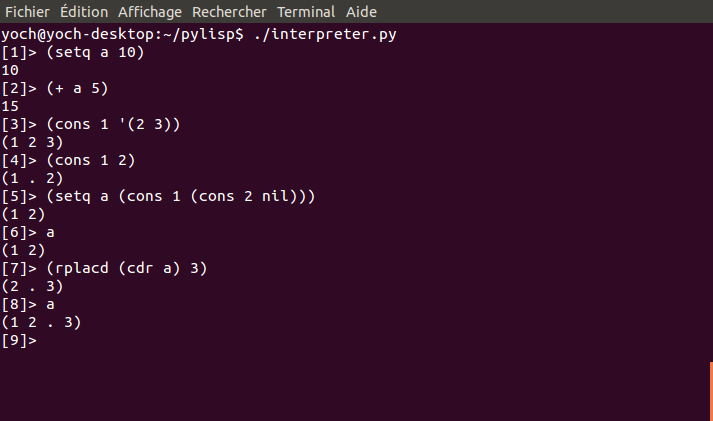
\includegraphics[width=1.\textwidth]{screen1.png}
\end{figure}

\subsection{Tests : test.py}
Il est assez facile d'effectuer des tests sur les deux composants principaux : parseur et interprète.
\\
Je me suis contenté d'écrire un fichier Python supplémentaire, avec des sources de petits programmes
Lisp sous forme de chaînes de caractères. Les programmes sont testés dans une boucle.

\paragraph{Échantillon de programmes testés}

\begin{minted}[linenos=false,
	       frame=lines,
               framesep=2mm]{python}
from lisp_lexer import lisp_lexer
from lisp_parser import lisp_parser

progs = [
#...
"(/ 5 0)",
"""
(defun fibo (n)
  (if (or (= n 0) (= n 1))
    n
    (+ (fibo (- n 1)) (fibo (- n 2))) ) )
(fibo 0)
(fibo 1)
(fibo 5)
(fibo 10)
(fibo)
(fibo 1 2)
""",
"""
(defun append (l1 l2)
  (if (not l1)
    l2
    (cons
      (car l1)
      (append (cdr l1) l2) ) ) )
(append '(1 2 3) '(4 5 6))
(append nil '(1 2))
(setq a '(8 9))
(setq b '(a b))
(append b a)
"""
]

for i, prgm in enumerate(progs):
    print('TEST N. {}'.format(i))
    ret = lisp_parser.parse(prgm, lexer=lisp_lexer)
    for e in ret:
        try:
            print('> {}'.format(e))
            print(e.eval())
        except Exception as err:
            print(repr(err))
            continue
\end{minted}

\paragraph{sortie} (on remarque que les erreurs sont bien détectées)

\begin{minted}[linenos=false,
	       frame=lines,
               framesep=2mm]{console}
TEST N. 13
> (/ 5 0)
Error: division by zero
TEST N. 14
> (defun fibo (n) (if (or (= n 0) (= n 1)) n (+ (fibo (- n 1)) (fibo (- n 2)))))
fibo
> (fibo 0)
0
> (fibo 1)
1
> (fibo 5)
5
> (fibo 10)
55
> (fibo)
Error: nombre d'arguments incorrect
> (fibo 1 2)
Error: nombre d'arguments incorrect
TEST N. 15
> (defun append (l1 l2) (if (not l1) l2 (cons (car l1) (append (cdr l1) l2))))
append
> (append (quote (1 2 3)) (quote (4 5 6)))
(1 2 3 4 5 6)
> (append nil (quote (1 2)))
(1 2)
> (setq a (quote (8 9)))
(8 9)
> (setq b (quote (a b)))
(a b)
> (append b a)
(a b 8 9)
\end{minted}

\section{Conclusion}
% principales qualités, principaux défauts et comment devrait-on poursuivre le travail

\paragraph{}
J'espère avoir montré que l'on peut, à peu de frais, implémenter un interprète Lisp basique en Python,
et que cet exercice pouvait également être l'objet d'une démarche plus générale de compilation dans
l'acceptation habituelle du terme.
\paragraph{}
Le travail présenté ici peut encore largement être amélioré, 
qualitativement (en ajoutant des mécanismes qui ne sont pas présents actuellement)
comme quantitativement (par exemple en réalisant un support étendu du langage).
Certains aspects des ajouts et modifications possibles ont été discuté dans le présent document.
\paragraph{}
Personnellement, je serais plutôt tenté de continuer en explorant d'autres branches du domaine de la compilation 
qui n'ont pas été traitées ici, comme la génération de byte-code, ainsi que l'optimisation
du code produit (optimisation de la récursion terminale entre autres).
\\
Tout ceci fera peut-être l'objet d'un travail ultérieur.

\section{Remerciements}
% 

Mes sincères remerciements vont à toutes les personnes qui m'ont aidé, directement ou indirectement à la
réalisation de ce projet, et en particulier :

\begin{itemize}
  \item à Gilles Bernard, qui m'a fait découvrir le langage Lisp à travers ses cours, et dont le programme \emph{Interlisp}
  étudié cette année a constitué une base de reflexion pour le présent projet.
  \item à Harald Wertz, spécialiste du langage Lisp, avec qui j'ai eu des échanges extrêmement riches et instructifs.
  \item à Jym Feat, que je n'ai malheureusement pas eu le plaisir de connaître, mais dont l'excellent
cours m'a donné envie d'aller encore plus loin.
\end{itemize}

\bibliographystyle{plain}
\bibliography{lisp_bib}

\end{document}
